\subsection{Data Collection}
\label{sec:data-collection}

\subsubsection{Questionnaire}
\label{sec:questionnaire}

Our main goal during the data collection process was to obtain GitHub Usernames along with as many answers to questions related to the subject of the recruitment process, an assessment of own skills as well as some additional information which could help in the reconstruction of results found in other papers. We have created a Google Form questionnaire and then posted it on two programming-related Facebook Groups.

In both groups, one can find people with a full range of professional experience but based on the activity (posts and comments), one of them is mainly characterized by highly qualified employees (Seniors) while the other seems evenly distributed.

\subsubsection{Parsing General GitHub Information}
\label{sec:github-info-parsing}

To collect data from GitHub, we used GraphQL Queries \footnote{GraphQL GitHub API: \url{https://docs.github.com/en/graphql}}. The query takes only the username on the input and on the output puts only the information precisely specified within the query itself. GraphQL Query is presented in the image below ~\textit{[ref: \ref{fig:graph-ql-query}]} and the output format can found in the listing right after underneath the figure ~\textit{[ref: \ref{lst:graphql-output-json}]}.

\begin{figure}[htp]
\centering
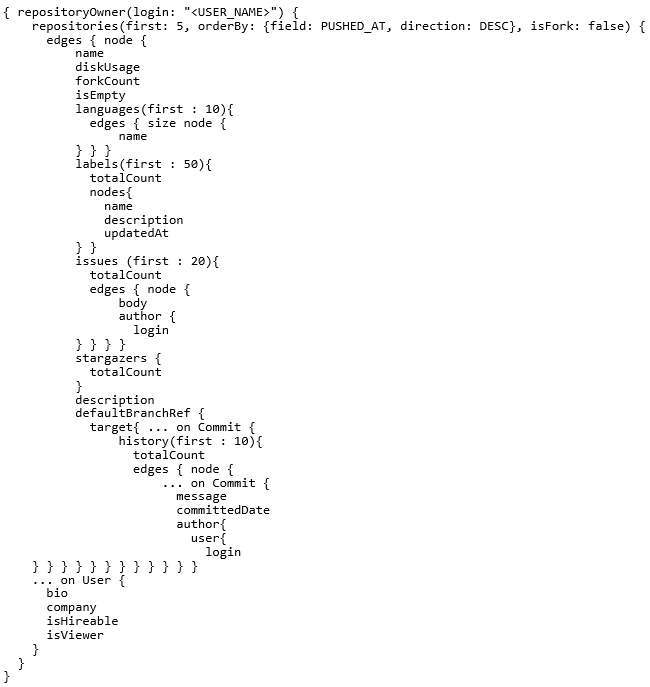
\includegraphics[width=11cm]{query}
\caption{GraphQL Query}
\label{fig:graph-ql-query}
\end{figure}

\begin{lstlisting}[language=Python, label={lst:graphql-output-json}]
FUTUREOUTPUT
\end{lstlisting} 

Requests were done within R script for every username, which was extracted from a GitHub link that was provided in the questionnaire. Unfortunately, not every participant provided a relevant link to the repository or even did not provide any. First, the script loads the questionnaire data and then for every username executes the request to GitHub API. In case of an invalid link, it returns blank data. After collecting data for every user who took part in the questionnaire, the script <TODO!: Co potem robi? Zapisujecie to do pliku CSV jako nowe kolumny?>.


\subsubsection{Parsing GitHub Repositories}
\label{sec:github-repo-parsing}

This part requires quite a bit of time to complete per just one single user. The time it takes to fetch and parse is mainly related to the number of repositories that a given user has as well as the contents which are in them. The script receives on input one single username and then it collects all repository names into a list. In the next step, all of these repositories are fetched from remote to the local computer so they can be checked via \emph{Mega Linter}. After collecting all of the repositories, \emph{Mega Linter} task is executed in each single one of them. When that is done, the script moves on to the merge task, which transforms all the generated \code{jsons} into one, single \code{json} file, so that it can be easily imported and accessed by the model in \emph{R}.


